\section{Experimental setup}
Experiments were executed on variations of the \textit{Cart-pole} environment and on variations of the \textit{Acrobot} environment.\\

In the 2-dimensional Cart-Pole environment, a pole is placed vertically on a cart. The goal in this environment is to keep the pole balanced vertically (i.e. keep the angle of the pole between thresholds) and to keep the cart between 2 borders.
The state is defined by 4 continuous-valued attributes: the position of the cart, the velocity of the cart, the angle of the pole and the angular velocity of the pole.
A discrete value of $1$ is given as a reward each time the pole is balanced and the cart is between bounds.
The episode ends either when these requirements are not fulfilled anymore or 200 steps have been executed.
An agent can either move left or right. It can't stay at its current position.
The environment is visualized in Figure~\ref{fig:cartpole}.
\begin{figure}[htb]
    \centering
    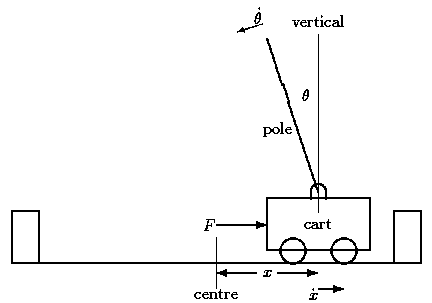
\includegraphics[width=.6\linewidth]{images/cartpole.png}
    \caption[Cart-Pole environment]{Cart-Pole environment. $F$ is the force applied to the cart when taking an action. $x$ is the distance of the cart from the center and $\dot{x}$ is its velocity. $\theta$ is the angle of the pole and $\dot{\theta}$ refers to its angular velocity. Source: \cite{grant1990modelling}.}
    \label{fig:cartpole}
\end{figure}
For executing the experiments, an implementation of this environment by \cite{Brockman2016OpenAIGym} was used.\\

The goal in the \textit{Acrobot} environment, visualized in Figure~\ref{fig:acrobot} is to swing up  the tip of 2 joined arms above a certain point \cite{spong1995swing}.
This can be done by applying a force on the joint between the 2 arms.
However, this force is not enough to fulfill the goal immediately. Instead, the actuator must apply force to the left and to the right to build up enough speed to get above the horizontal threshold.
The state consists of the angle and angular velocity of both arms. One can either move the joint clockwise, counter-clockwise or do nothing.
An episode stops either when the tip of the outermost arm is above the threshold or when 500 steps have been executed in the episode.
The goal is to minimize the amount of steps necessary to reach the threshold.
\begin{figure}[htb]
    \centering
    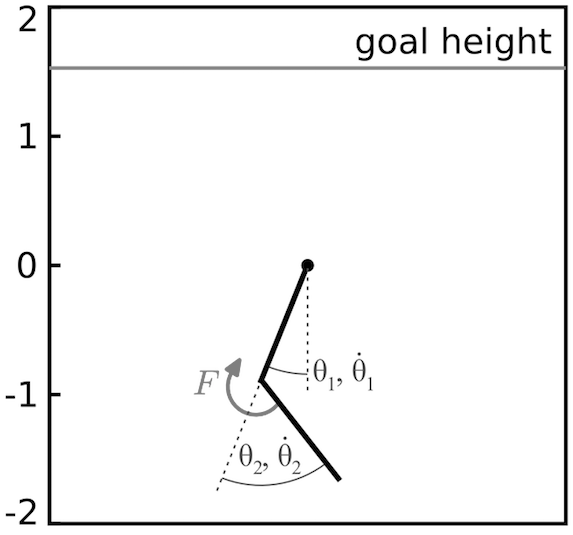
\includegraphics[width=.7\linewidth]{images/acrobot.png}
    \caption[Acrobot environment]{Acrobot environment. $\theta_1$ and $\dot{\theta_1}$ are respectively the angle and angular velocity of the arm attached to the central fixed point. $\theta_2$ and $\dot{\theta_2}$ are respectively the angle and angular velocity of the outermost arm. Source: \cite{fremaux2013reinforcement}}
    \label{fig:acrobot}
\end{figure}

In the experiment, first a number of environments are randomly generated. We try to learn with both 5 and 10 environments.
The environment for each task can differ for a predefined number of attributes, of which the values can each be in a certain range. For a cart-pole task, these are the mass of the cart, the mass of the pole and the length of the pole.\\
Then a number of source tasks were learned that can update both the shared knowledge base and their own sparse representation. After a number of epochs, i.e. updates to these variables, we stop with learning these tasks.
Instead, we learn to solve a new task, the target task, for which we hadn't learned its sparse representation yet. Here however, only the sparse representation can be updated and not the shared knowledge base.\\
This learning process is repeated 100 times, each time using a different set of environments and thus problems to solve.\\
Afterwards the rewards are averaged over all the runs.\\
Trajectories for both sets of tasks contained of maximally 200 or 500 steps depending on the type of environment. This could be less in case the environment was in an end state. In case of the cart-pole environment, this can mean for example that the cart tried to cross the left or right border or that the pole fell down.\\
Hyperparameters, such as the learning rate of neural networks, were chosen by iteratively executing the previously mentioned experiment. Possible values for each hyperparameter were chosen manually.
